\documentclass[a4paper,11pt]{article}
\usepackage[margin=2cm]{geometry}
\usepackage{anysize}
\usepackage[pdftex]{graphicx}
\usepackage{url}
\usepackage{listings}
\usepackage{textcomp}
\usepackage{wrapfig}
\usepackage{color}
\usepackage{subfig}
\usepackage{fancyhdr}
\usepackage[nodayofweek]{datetime}
\usepackage[small,compact]{titlesec}
\usepackage[pdfborder=0]{hyperref}
\longdate

\setlength{\parskip}{10pt} 
\setlength\parindent{0pt}
\pagestyle{fancyplain}
\fancyhf{}
\lhead{\fancyplain{}{Machine Learning CBC}}
\rhead{\fancyplain{}{\today}}
\cfoot{\fancyplain{}{\thepage}}


\title{395 Machine Learning\\\Large{--- Assignment 2 ---}}
\author{Group 7\\Porfyrios Vasileiou, Afxentios Hadjiminas, John Flanagan.\\
       \{pv311, ah2411, jf311.\}@doc.ic.ac.uk\\ \\
       \small{CBC helper: Ioannis Marras}\\
       \small{Course: CO395, Imperial College London}
}


\begin{document}
\maketitle

\section{Introduction}

\section{Acquired decision trees}
    \begin{figure}[!h]
    \centering
    \subfloat[Anger (1)]{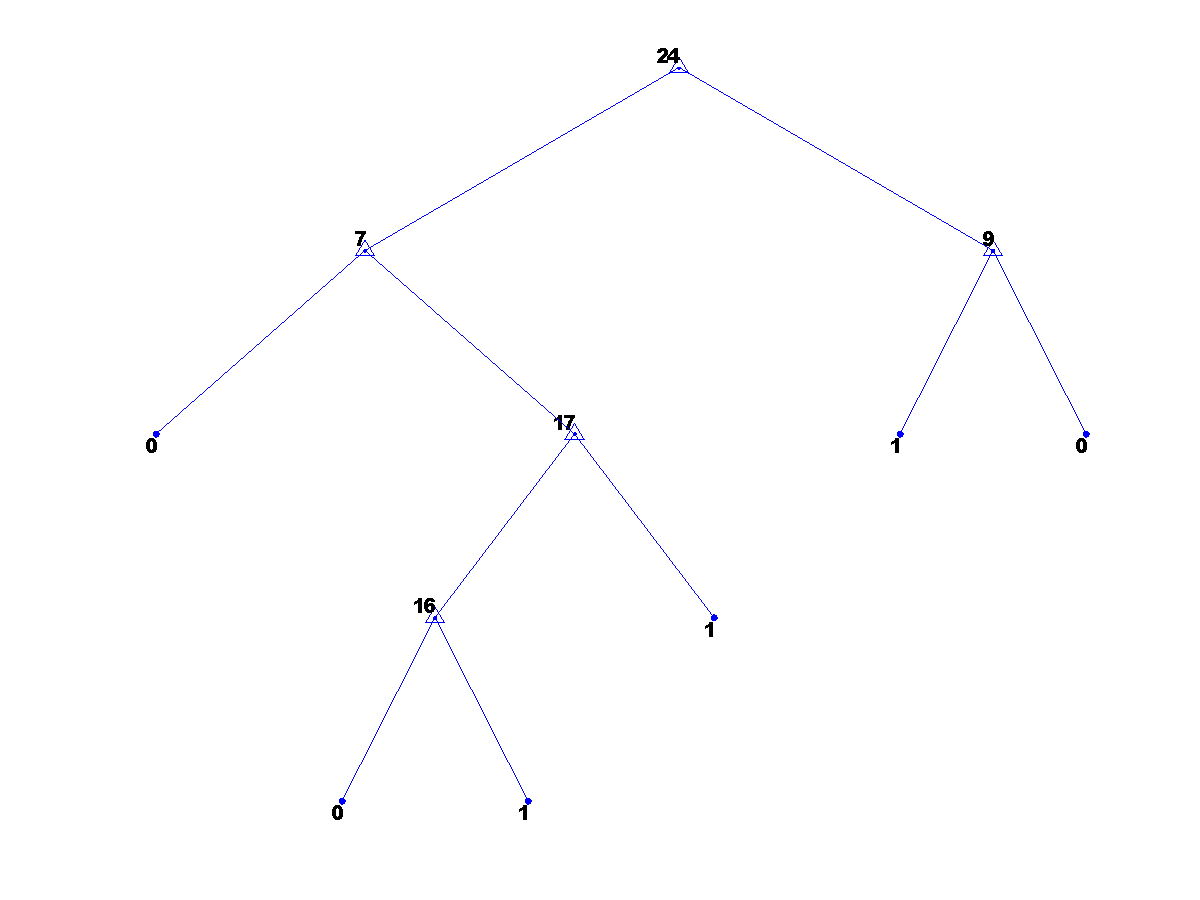
\includegraphics[width=0.5\textwidth]{tree1.pdf}}                
    \subfloat[Disgust (2)]{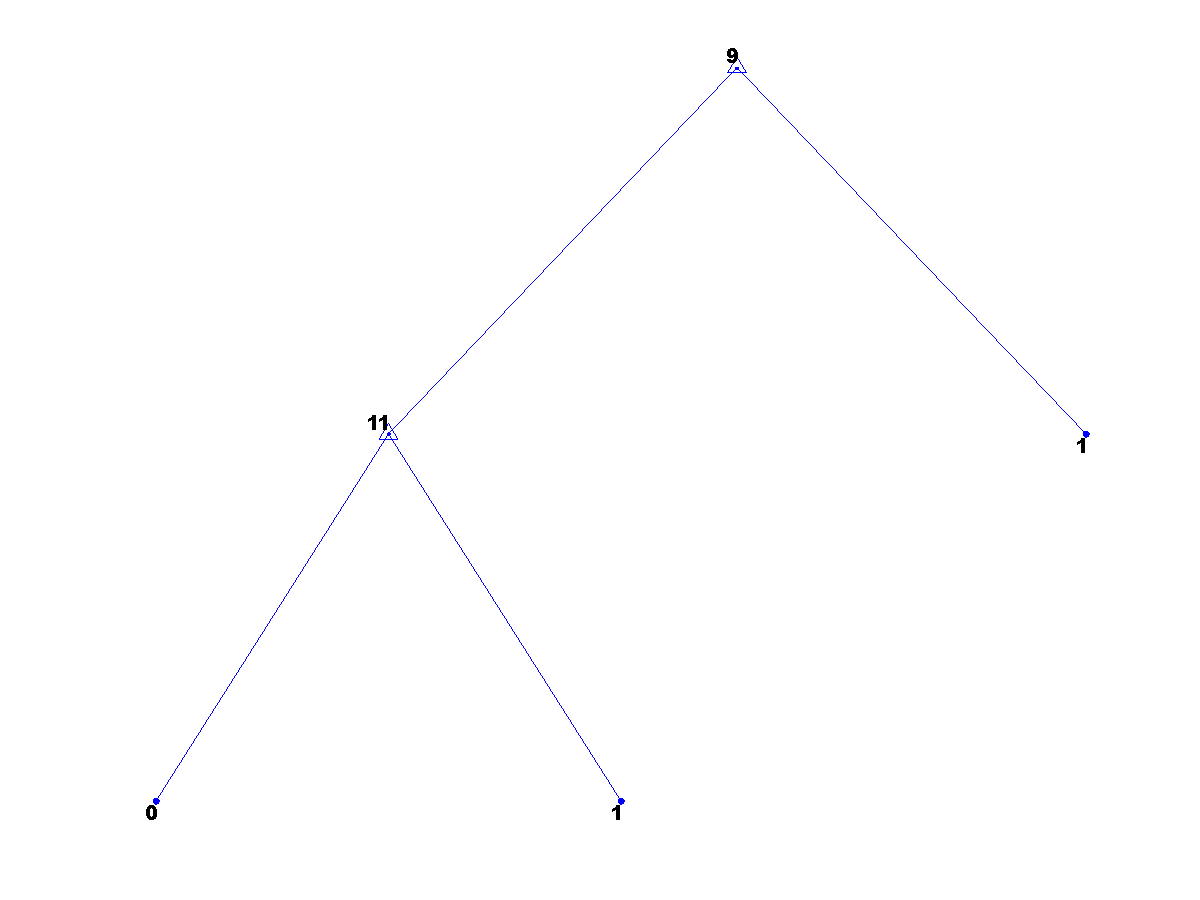
\includegraphics[width=0.5\textwidth]{tree2.pdf}}
    
    \subfloat[Fear (3)]{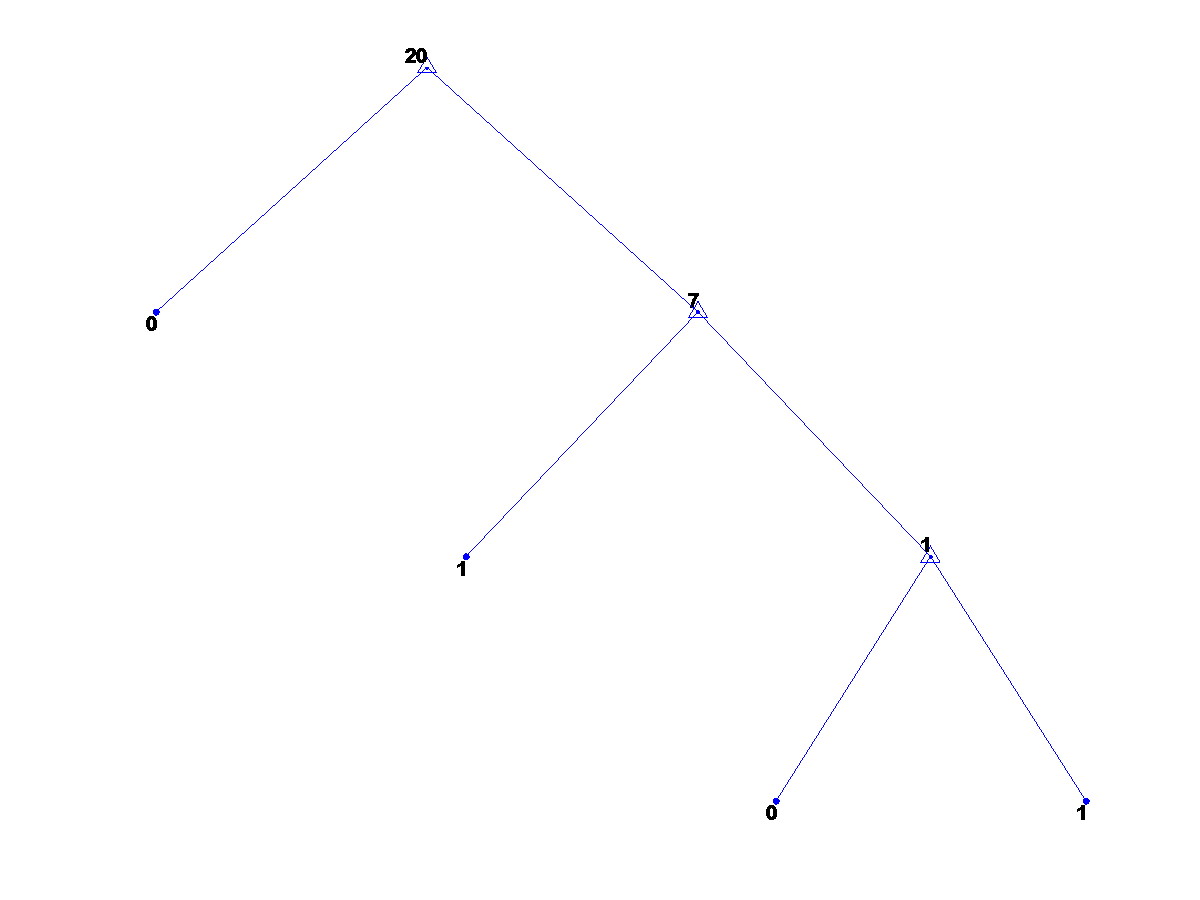
\includegraphics[width=0.5\textwidth]{tree3.pdf}}
    \subfloat[Happiness (4)]{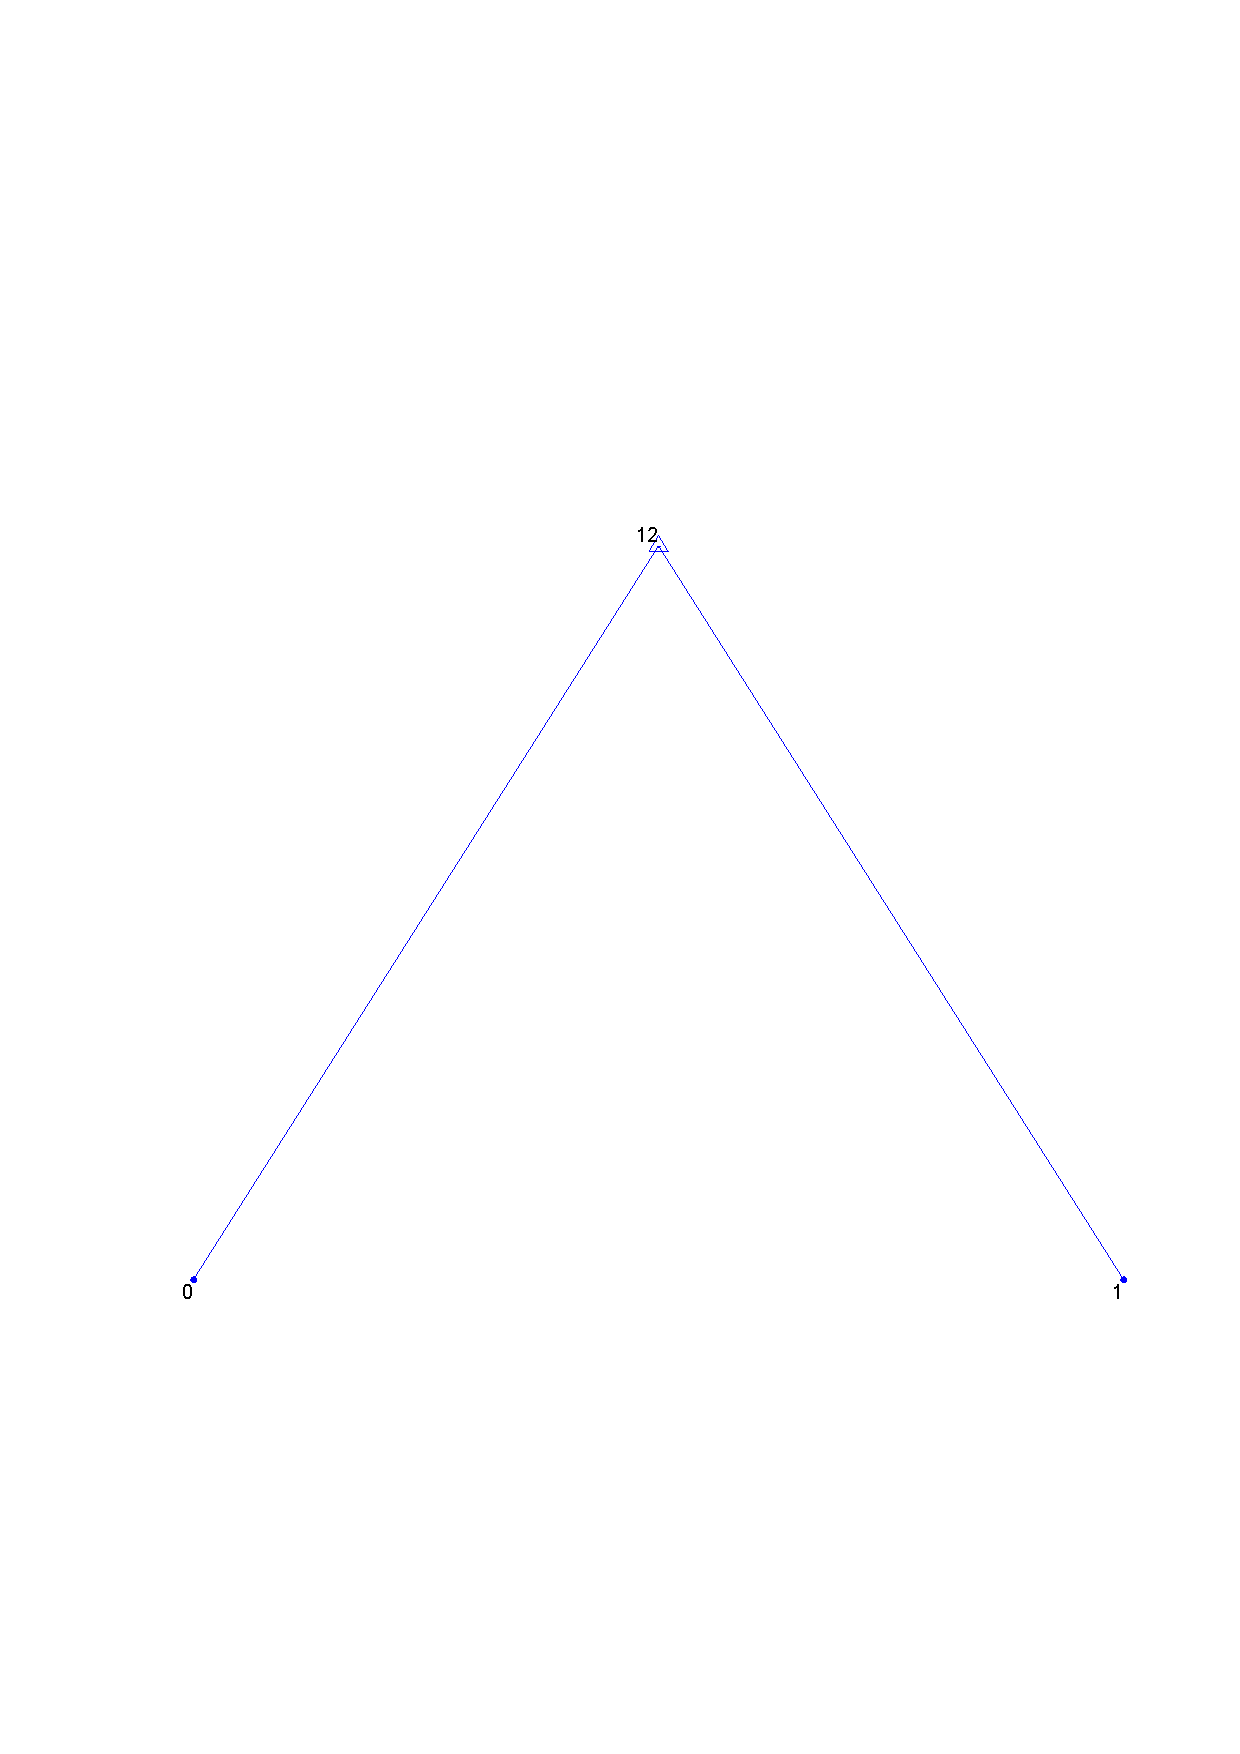
\includegraphics[width=0.5\textwidth]{tree4.pdf}}
    
    \subfloat[Sadness (5)]{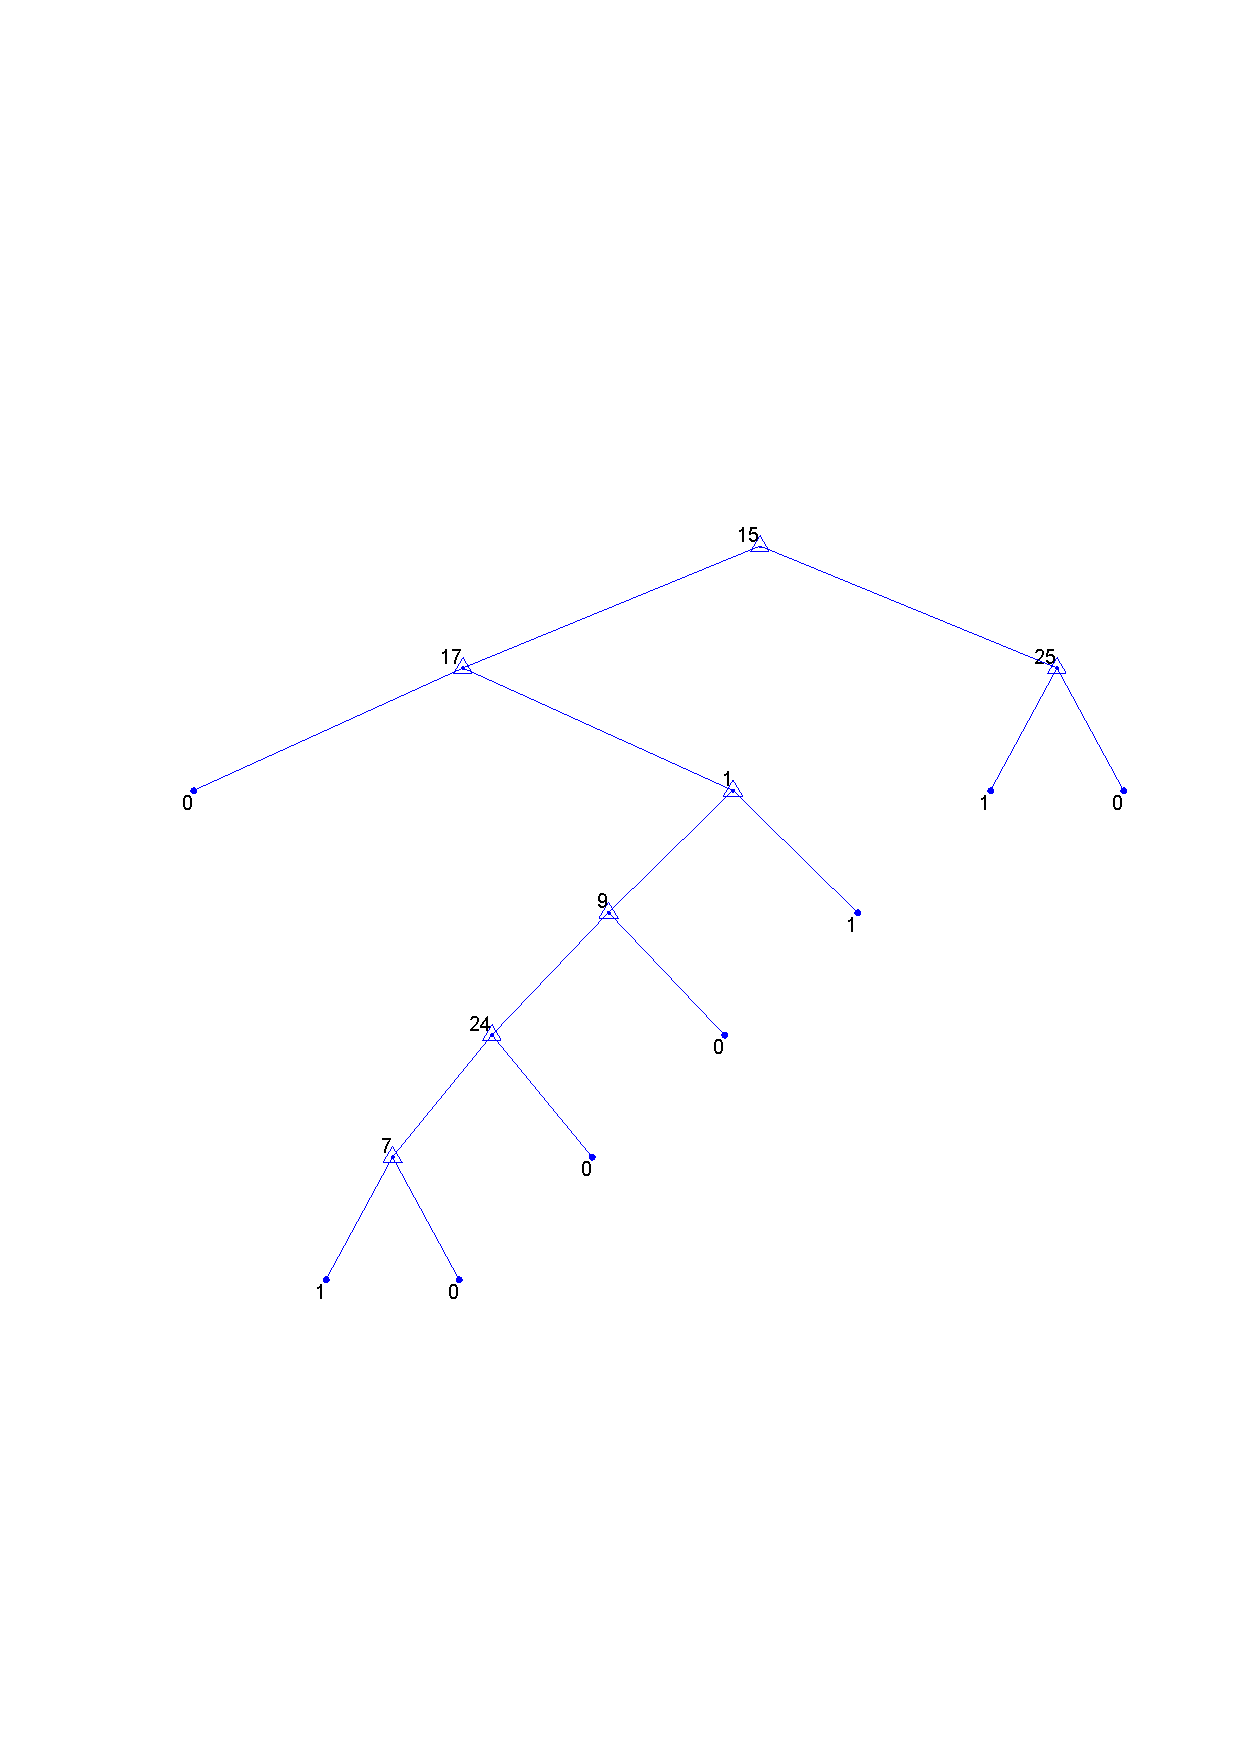
\includegraphics[width=0.5\textwidth]{tree5.pdf}}
    \subfloat[Surprise (6)]{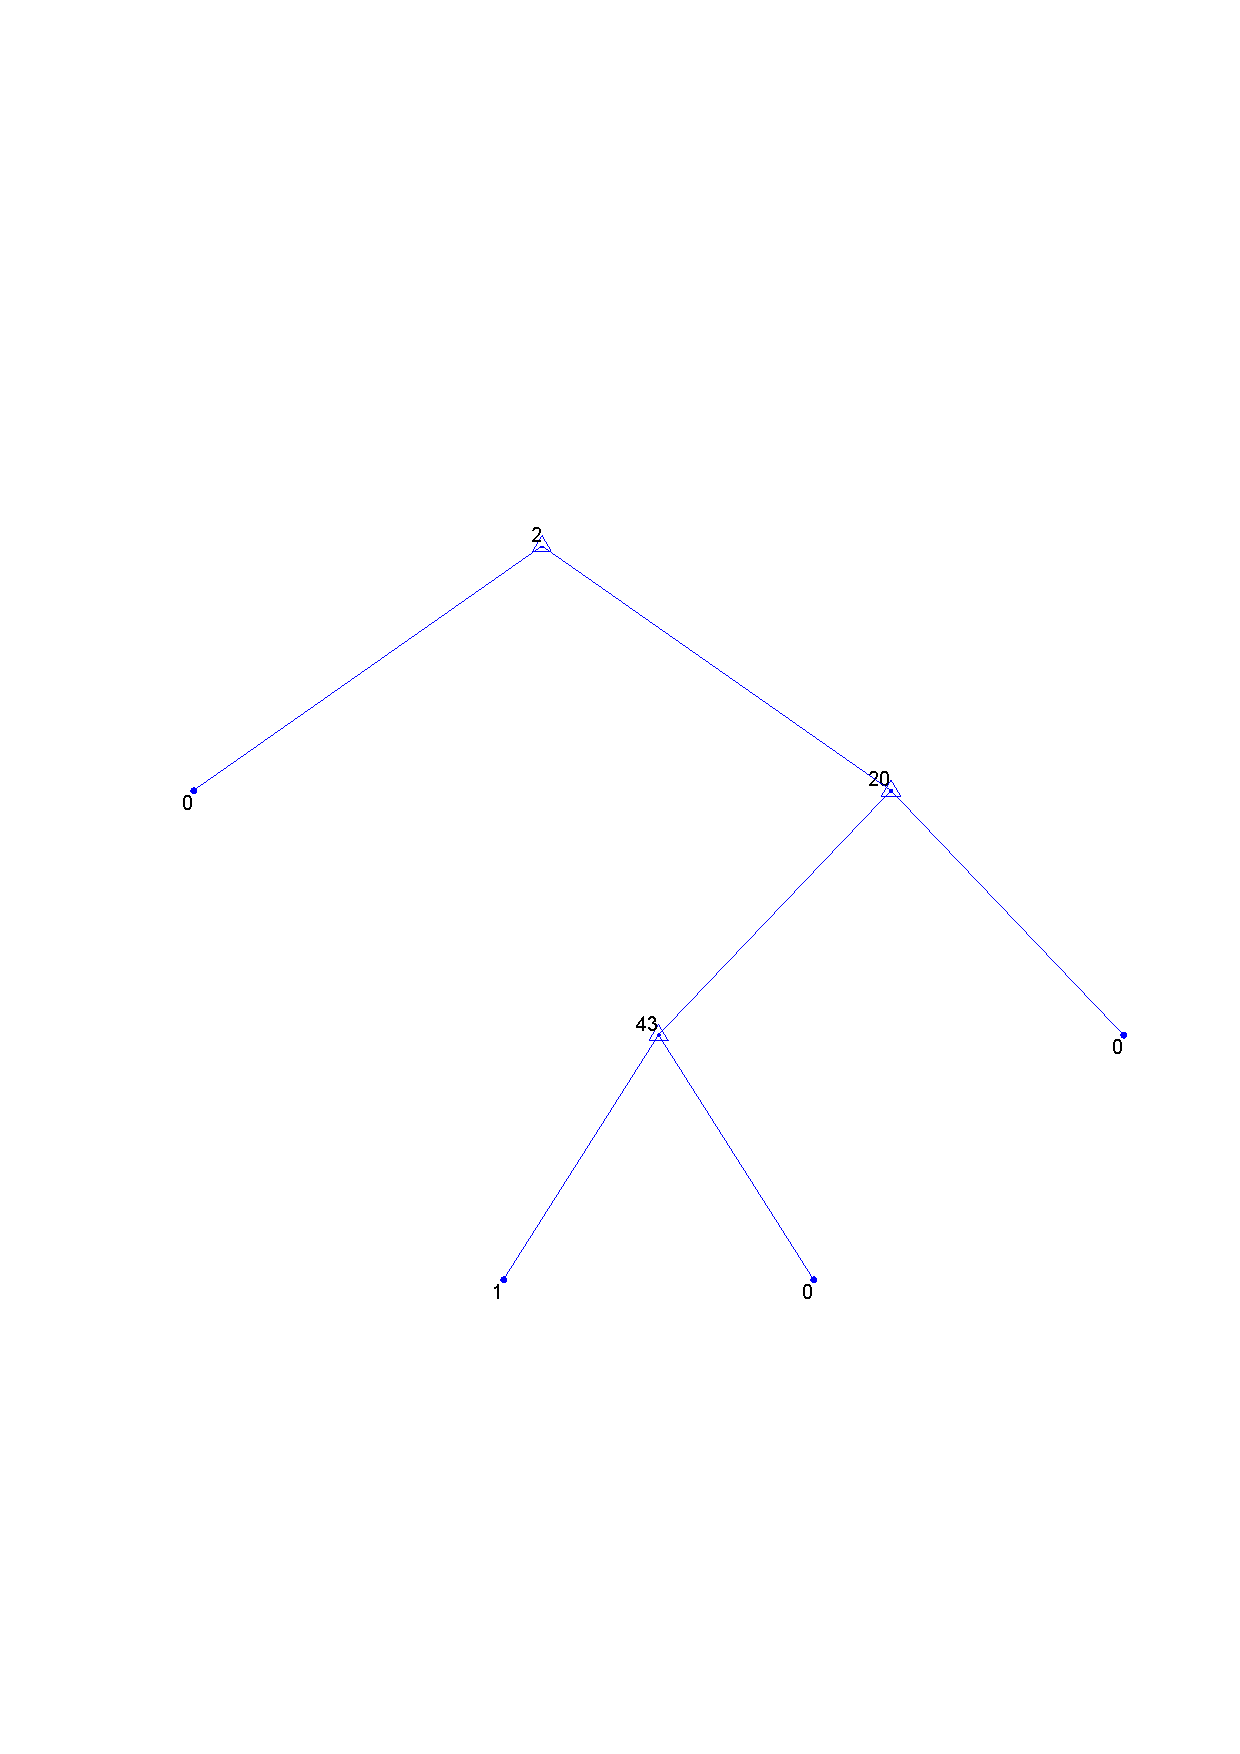
\includegraphics[width=0.5\textwidth]{tree6.pdf}}
    \caption{Acquired decision trees for each emotion}
    \label{fig:decisionTrees}
\end{figure}



\section{Single emotion per exampe}

\section{Ambiguity}

\section{Cross validation classification results}
    \subsection{Confusion matrix}
    \begin{center}
    \begin{tabular}{ | l || c | c | c | c | c | c | }
    \hline
          & 1 & 2 & 3 & 4 & 5 & 6 \\ \hline \hline
        1 & 9 & 1 & 1 & 0 & 1 & 0 \\ \hline
        2 & 0 & 21 & 1 & 0 & 0 & 0 \\ \hline
        3 & 2 & 0 & 4 & 0 & 1 & 0 \\ \hline
        4 & 0 & 0 & 0 & 24 & 0 & 0 \\ \hline
        5 & 0 & 1 & 0 & 0 & 9 & 2 \\ \hline
        6 & 0 & 0 & 0 & 0 & 0 & 23 \\ \hline
    \end{tabular}
\end{center}


\section{Pruning}
    \subsection{\emph{pruning\_example} function}

%\pagebreak	
%\section{References}
%	\vspace{-20pt}
%	\def\refname{}
%	\bibliography{references}
%	\bibliographystyle{plain}

\end{document}
